% 1_introduction.tex

\cleardoublepage
\chapter{Introduction}

  	
  	
  	In recent years, the space sector has seen a significant shift in the paradigm of space launch system design. 
  	The sector has moved towards privatisation, with new and innovative launch systems competing to offer the most cost-efficient and reliable launches. 
  	The Sector has also seen a split between those who produce large satellite launchers and those who produce small launchers.
  	For large payload launchers, reusability is a major focus in the design of new launch systems, with the purpose of making a launch system cost efficient over multiple launches. 
  	For small payload launchers, reusability is more complex than for large launchers, as the additional systems necessary for reusability add a larger fraction of system mass, and require a proportionally larger fuel mass. 
  	Consequently, the focus of small launch system design is currently on producing expendable launch systems as cheaply and efficiently as possible, using state of the art technologies such as 3D printing to expedite the process.
  	However, if reusability is able to be successfully integrated into small launch system design, it has the potential to increase the cost efficiency and launch flexibility, potentially opening up the small satellite market significantly. 
  	
  	
  	
  	A potential candidate for integrating reusability into small satellite launch systems is the use of airbreathing engines.
Airbreathing engines produce higher specific impulse than rockets, and require far less propellant to be carried on-board a launch vehicle.  
 	The use of airbreathing engines for reusability has particular applicability to small satellite launchers. 	 
  	The higher efficiency and reduced propellant mass of airbreathing vehicles allows the additional mass of the systems necessary for reusability to be mitigated. An airbreathing vehicle can be designed in a similar fashion to a conventional aircraft, with wings, stabilisers and ailerons.
  	
  	The primary engines in consideration for launch vehicles are ramjet and scramjet engines. These engines offer good efficiency and have operational regimes which allow them to effectively accelerate a launch vehicle over a range of Mach numbers. 
  	Ramjets and scramjets rely on the high velocity of the aircraft to compress the flow of air entering the engine before combustion.  Ramjets slow the air to subsonic speeds and are suited to operation at low Mach numbers, whereas scramjets keep the flow supersonic throughout, and operate within the hypersonic regime, above Mach 5. 
  	The strict operational regime of these engines means that a launch system cannot be solely powered by airbreathing engines. Rocket power is necessary for at least the exoatmospheric portion of the trajectory, and is necessary also to accelerate the ramjet or scramjet to minimum operational speed.
  	As a result, the designs of airbreathing launch systems are necessarily partially-airbreathing, usually separated into multiple stages to increase weight efficiency. 
  	 
  	 The design of the trajectory of a partially-airbreathing launch system is extremely important to its performance. 
  	   The airbreathing engines of a ramjet or scramjet-powered stage require high dynamic pressure to operate effectively, and airbreathing engines are generally designed for high lift-to-drag. Conversely, rocket-powered stages produce more thrust at higher altitude, and are generally designed for weight efficiency. For these launch systems, the various stages and engines involved during launch require trade-offs in engine efficiency and thrust generation, stage mass, and vehicle aerodynamics. These factors require the launch trajectory of the system to be thoroughly simulated and optimised, to ensure that the launch vehicle is operating effectively. 
 	  

  Calculating the optimal trajectory for a space launch system is an integral part of the preliminary vehicle and mission design process. An optimal trajectory calculated without predispositions can offer valuable insights into the performance of a launch vehicle, and drive future design decisions. Calculating the optimal trajectory profile for a launch system typically requires the use of optimal control theory. Optimal control theory is a general set of techniques which find a control law to maximise a given metric of a system. For a launch vehicle, optimal control allows the best possible payload-to-orbit to be calculated in simulations during design. 
Optimal control theory allows a trajectory to be calculated in which the flight path of each individual vehicle is considered simultaneously to produce a maximum-payload trajectory. 
This concurrent optimisation is particularly important for launch systems incorporating airbreathing engines, where the performance of each vehicle is thoroughly different. 
Optimal control is able to produce an optimised trajectory which satisfies the specific structural and flight constraints of the vehicle being simulated. These constraints allow for the physical limitations of the vehicle, such as heating and structural loading limits, to be imposed. These constraints also allow any necessary mission conditions to be established, such as reaching orbital velocity and achieving fly-back. 
  
  
  	   This study applies optimal control theory to a three stage rocket-scramjet-rocket launch system being developed by The University of Queensland, designated The SPARTAN. This launch system is designed to be partially reusable, with at least the second stage scramjet vehicle flying back to the initial launch site. 
  	   In previous studies it has been assumed that the optimal trajectory for the scramjet powered vehicle is at its
  	   maximum dynamic pressure and all other trajectory stages have conformed to this assumption.
  	   This study will develop an optimal trajectory profile for The SPARTAN, with the aim of producing an optimal
  	   trajectory profile which may be applied to any rocket-airbreathing-rocket system for delivering small
  	   satellites to Earth orbit. 
  	   
  	  	\begin{figure}[ht]
  	  		\centering
  	  		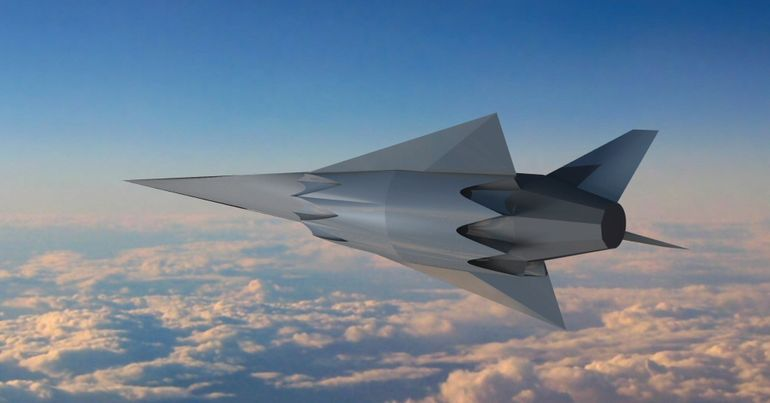
\includegraphics[width=0.7\linewidth]{figures/1_introduction/project-spartan}
  	  		\caption{The scramjet-powered second stage of the SPARTAN CITATIONXX.}
  	  		\label{fig:project-spartan}
  	  	\end{figure}
  	  	

  \section{Research aims}

    The aim of this work is to apply state of the art numerical optimisation techniques to the trajectory of a rocket-scramjet-rocket small satellite launch system. The purpose of this optimised trajectory is to maximise the payload-to-orbit capabilities of the launch system, thereby also maximising the cost efficiency of the system. The optimised trajectory must take all three stages into account, as well as the fly-back of the second stage scramjet accelerator. 
    The optimal trajectory result will be investigated for robustness to indicate whether it is applicable for general multi-stage rocket-scramjet-rocket launch systems. The optimised trajectory of vehicle configurations with resized third stages will be studied to give insight into the impact of the relative sizing of the launch system. 
 
    
\vspace*{10pt}
    \noindent These aims will be achieved through the following objectives:
    \begin{enumerate}
    	 \item \emph{Development of a detailed design and simulation for a rocket-scramjet-rocket launch system.}
    	 
    	   For an optimal trajectory to be calculated, a detailed launch system design and robust simulation are required. This design must be representative of a standard rocket-scramjet-rocket launch system for the optimal trajectory results to be generally applicable.\\

\item \emph{Calculation of a maximum payload-to-orbit trajectory using optimal control.}

The trajectory of a multi-stage rocket-scramjet-rocket system is sensitive to a multitude of factors. Optimal control techniques allow a maximum-payload trajectory to be calculated with few assumptions as to the general shape of the trajectory. \\
    	
      \item \emph{Evaluation of the robustness of the optimal trajectory, by investigation into the sensitivity of the solution to variation in vehicle aerodynamic parameters.} 

The robustness of the optimal trajectory indicates whether the calculated trajectory shape is applicable to multiple rocket-scramjet-rocket designs. \\

      \item \emph{Investigation into the effects of varied third stage sizing.}

The relative sizing of the stages in a launch system can have a large effect on the payload cost efficiency of the system. Optimising the trajectory for multiple configurations shows how the maximum payload-to-orbit varies compared to the proportional size of the expendable stages of the launch system. \\


    \end{enumerate}

  \clearpage
  \section{Thesis outline}

    

    \subsubsection*{Chapter 2 - Literature Review}

      A review of literature related to the different aspects of this thesis is presented. The theory behind scramjet propulsion is outlined, followed by a background of reusable and small satellite launch systems. A review of the trajectories of partially-airbreathing launch systems is presented, comparing the optimised trajectories of various conceptual vehicles. An overview of optimal control theory is presented, with particular emphasis on the pseudospectral method of optimal control, which is employed within this study. Lastly, an overview of the optimal control and aerodynamic solvers which are used in this study is presented.
      

    \subsubsection*{Chapter 3 - Launch Vehicle Baseline Design}

      The design, aerodynamics and engine models of all three stages are detailed. The SPARTAN scramjet-powered stage is presented first, followed by the first and third stages, due to the external scramjet vehicle design being taken from prior work. The design of each stage is presented, followed by the propulsion model used, and finally the simulated aerodynamic characteristics. 
      
      
      \subsubsection*{Chapter 4 - LODESTAR}
      
      The method used for the simulation and optimisation of the trajectory is detailed, including the creation of the trajectory analysis program, LODESTAR, which has been created for this study. The specifics of the optimal control methodology used are presented, along with relevant examples. The simulation methodology is detailed, along with the construction of the optimal control simulation. The specific set-up of the optimal control program is detailed for each trajectory stage, specifying the costs and constraints which drive the optimal control solver. Finally, the methods for validating the final solutions are specified.
      
      \subsubsection*{Chapter 5 - Optimised Trajectory}
      
      The results of the trajectory optimised using LODESTAR are presented. The ascent of the SPARTAN and third stage rocket are optimised along with the fly-back of the SPARTAN, for maximum payload-to-orbit. The first stage rocket is optimised to the first-second stage separation point, for minimum fuel usage. The optimal trajectory is analysed. It is found that a pull-up at the end of the scramjet stage trajectory significantly improves payload-to-orbit. It is also found to be necessary to reignite the scramjet engines during the return flight of the scramjet accelerator to achieve fly-back. The scramjet stage banks during acceleration to lessen fuel consumed during the return flight.
      
      \subsubsection*{Chapter 6 - Trajectory Sensitivity Study}
      
      The sensitivity of the optimal trajectory to variation in the aerodynamic coefficients and engine properties of the scramjet stage are studied. It is found that $\pm$10\% variation in L/D, specific impulse, and maximum allowable dynamic pressure produce very similar optimal trajectory shapes, indicating that the optimised trajectory is robust across scramjet vehicle designs. 
      
      \subsubsection*{Chapter 7 - Third Stage Sizing Study}
      
      The effects of variation in the size of the third stage rocket are investigated. The third stage rocket is varied in length and width by $\pm$10\%, along with corresponding changes to the internal design of the SPARTAN. \textcolor{red}{Results of this section are currently being determined.} 
      
     
      

    \subsubsection*{Conclusions}

      The body of this thesis concludes by summarising the most significant findings from this work. Recommendations for future work are made. 